\documentclass[
%% TIKZ_CLASSOPTION %%
tikz
]{standalone}
\usepackage{amsmath}
\usetikzlibrary{matrix}
%% EXTRA_TIKZ_PREAMBLE_CODE %%
\begin{document}
%% TIKZ_CODE %%
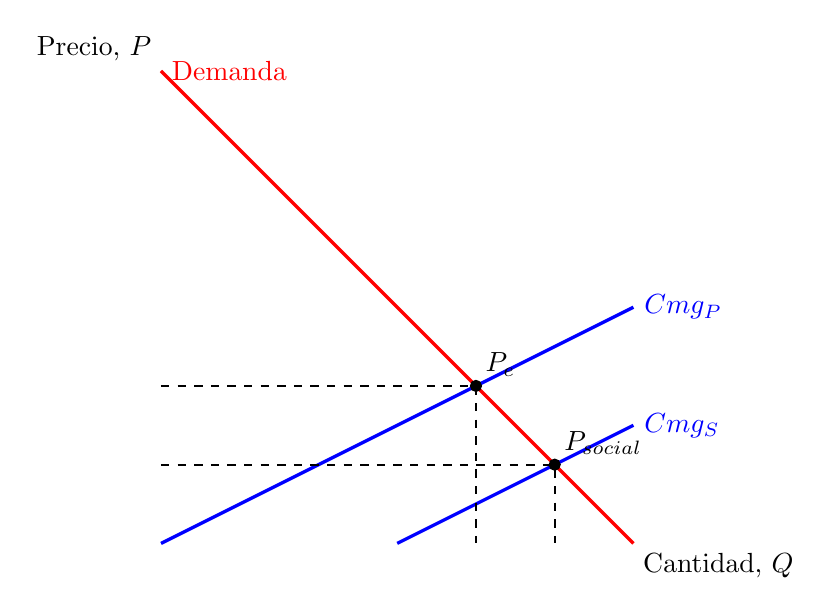
\begin{tikzpicture}
% Supply and demand curves
\draw[red, very thick] (6,0) -- (0,6) node[right] {Demanda};
\draw[blue, very thick] (0,0) -- (6,3) node[right] {$Cmg_{P}$};
\draw[blue, very thick] (3,0) -- (6,1.5) node[right] {$Cmg_{S}$};

% Dashed lines
\draw[black, dashed, thick] (0,2) -- (4,2) -- (4,0);
\draw[black, dashed, thick] (0,1) -- (5,1) -- (5,0);

% Coordinate points
\filldraw[black] (4,2) circle (2pt) node[above right] {$P_{e}$};
\filldraw[black] (5,1) circle (2pt) node[above right] {$P_{social}$};

% Labels
\node[below right] at (6,0) {Cantidad, $Q$};
\node[above left] at (0,6) {Precio, $P$};
\end{tikzpicture}
\end{document}
